\chapter{Discussion}
In this section, the methods and models implemented for the research will be discussed and compared. First, the downsampling method will be examined. After this, the seven models will be reviewed beginning with the least successful (\ac{cnn} classification) and working up to the most successful (polynomial regression on key values and features).

\section{Downsampling} \label{sec:disc:downsampling}
The downsampled flight data was highly successful in terms of data reduction, flight comparability and compatibility with fixed-length inputs to neural networks. However, this representation also has several drawbacks.

Firstly, while a data loss of 1.2\% is low, it does not rule out that a significant loss of \textit{information} took place. If, for the sake of argument, most damage occurred during the descent phase, the shape of the downsampled data in Figure \ref{fig:0815_ds} would suggest that the data essential to predicting the damage had been lost. % TODO: What is reconstruction error of just this phase?
The peaks of most large fluctuations during this phase are dampened due to using an insufficient number of data points to approximate the data.

Secondly, in the downsampled time series data, although the amplitudes of most flight manoeuvres and parameter fluctuations are approximated well, all relative temporal information is lost. Without finding a suitable means of incorporating the corresponding time data (the array of indices \(K\) from Section \ref{sec:recon_err}) into the models, the model is completely oblivious to the length of each flight and the lengths of the phases within it. Furthermore, because the downsampling is carried out separately for each parameter, downsampled time points (except at phase boundaries) across the parameters are not necessarily aligned. This information may not be as valuable as phase duration for damage prediction, but it is still a loss that could be avoided. Without this temporal information, neural network-based models can only learn from data amplitudes and their order.

One possibility for improving results of time series models may therefore be increasing the length of downsampled time series to reduce the loss of data and information.

Finally, many fluctuations in NH, T30 and P30 take place during the descent phase (Figures \ref{fig:high_low_dmg_NH}, \ref{fig:high_low_dmg_P30} and \ref{fig:high_low_dmg_T30}). These fluctuations are approximated by only 10 time points in the downsampling. The nature of this phase and the downsampling means that the values in the downsampled data are generally either high or low and not in between, as shown by the diamond-shapes resulting from the fluctuations. While these are ideal attributes for a \ac{cnn} to learn, they are precisely the type of attribute that will `confuse' an \ac{mlp}: While an average NH value at time point 7 would be expected to correspond with average damage (Figure \ref{fig:dmg_violin_NH}), no conclusions could be drawn from an average value at time point 60 during the descent phase, since this could be the peak of a low-damage flight or the trough of a high-damage flight.

An optimisation in this respect could therefore involve downsampling the descent phase such that the peaks and troughs of fluctuations are aligned, much in the same way as is visible at (and between) time points 65 and 66 of Figures \ref{fig:high_low_dmg_NH}, \ref{fig:high_low_dmg_P30} and \ref{fig:high_low_dmg_T30}.

\section{Convolutional Neural Network}
The \ac{cnn}, despite its consistent presence in state-of-the-art models in the field of computer vision, did not perform well on the time series data.

Each InceptionTime-based model, trained for 500 epochs with all default hyperparameter values as recommended by \citet[]{fawaz_inceptiontime_2019}, took approximately 4 hours to train. Considering the training time and the number of trainable parameters (507\,207) they contain, one would be forgiven for expecting better results.

\subsection{Time Series Classification}
Results from the classification problem show that the model is capable of correctly labelling a flight as one of four damage classes in fewer than half of cases. In Figure \ref{fig:classif_pred_hist} we saw the feature-wise absolute error: most flights are either correct or wrong by one class. While this appears promising, in terms of correctly classified flights, the model does not perform substantially better than simply guessing.

The accuracy of classification was likely hindered, as has been mentioned, by the lack of ordinality in classification and by information loss at the downsampling stage. Furthermore, a rule of thumb \cite[]{goodfellow_deep_2016} is to supply approximately 5\,000 training samples per class to be predicted; the complete dataset in this thesis contains 10\,534 training samples, about half of the number recommended for an acceptable level of accuracy in four classes. This severely limits the classification model in terms of scalability

Classification, while an interesting approach, should not be pursued further for damage prediction.

% \begin{figure}
%     \centering
%     \includegraphics[width=\textwidth]{pred_bar_complete}
%     \caption{\label{fig:classif_pred_bar} Bar plot of class predictions from the \ac{cnn} classification model on the complete dataset.}
% \end{figure}

\subsection{Time Series Regression}
Results from the \ac{cnn} time series regression are promising. Figure \ref{fig:incep_mts_reg_scatter} shows that the model is moderately capable of recognising and predicting a trend in damage from flight data. This ability is most visible in the plots of features 1 to 3. Features 6 and 7, on the other hand, illustrate the model's inability to extrapolate beyond the training data: one flight with over 13 cycles of damage in both features was predicted to consume fewer than 4. No flights in the training data breached 8 cycles, so the model was not equipped to predict damage beyond this value.

Interestingly, \(R^2\) and MHR were best from the model trained on the greatly reduced dataset. This means that the model could be scalable: If accuracy for the InceptionTime regressor can be improved, the model could still be a good candidate for use on a minimal dataset.

\section{Multilayer Perceptron}
The results and plots from \ac{mlp} models show that it is also clearly capable of recognising a trend in the data. The model performs well on all three datasets in all three sizes.

The training time for an \ac{mlp} ranged from approximately 15 seconds (key value datasets, with and without features) to slightly over one minute (\ac{mlp}), several orders of magnitude faster than the \ac{cnn} models.

\subsection{Time Series Regression}
Visually (Figure \ref{fig:mlp_mts_reg_scatter}), the performance of the \ac{mlp} is comparable to that of the InceptionTime regressor: It clearly regognises a trend in features 1 to 3, but struggles to keep the spread of its predictions for the 99.5\% of flights under 2 cycles within the tolerance. Its hit rate is highly comparable with that of the InceptionTime regressor, but its visibly wider spread results in a poorer \(R^2\) score for all dataset sizes.

\subsection{Key Value Regression}
The \ac{mlp}'s performance on the key value dataset is comparable to its performance on the concatenated time series dataset in terms of MHR. Higher damage values tend to be predicted with a greater error, which explains its poor \(R^2\) scores in the smaller dataset sizes.

The anomalous highest-damage flight in features 6 and 7 is predicted with far greater success, as visible in Figure \ref{fig:mlp_keyval_reg_scatter}, and it is correctly predicted to be the most damaging flight. The feature 7 prediction is marginally above the maximum damage from the training dataset, suggesting that the \ac{mlp} regressor is capable of extrapolating --- albeit not by a great amount in this case --- when trained on key values.

Interestingly, the scatter plot shows a much better performance in terms of spread on features 4 and 5 in comparison to the time series model. Unfortunately, the spread of the predictions increases greatly as the dataset is reduced, for which reason using an \ac{mlp} with the input values contained in this dataset is not recommended for further research.

\subsection{Regression on Key Values and Features}
According to Table \ref{tab:model_summary}, this model is consistently second best. It scores very highly in both MHR and \(R^2\), with one close \(R^2\) win on the reduced dataset.

Visually (Figure \ref{fig:mlp_keyvalfeat_reg_scatter}), the predictions come very close to the Cycle Counter values, and the model makes a near-perfect prediction of even the anomalous flight.

With its short training time, the \ac{mlp} combined with this dataset is highly suitable for further consideration in the research.

\section{Polynomial Regression}
The polynomial regressor with a polynomial degree of 3 required less than one second to train on the complete dataset.

The results from this model and the \ac{mlp} confirm findings by \citet[]{cheng_polynomial_2019}: the \ac{mlp} essentially performs the same function as a polynomial regression, but the latter has benefits in performance and simplicity. The only hyperparameter requiring attention and optimisation in a polynomial regression model is the polynomial degree; in an \ac{mlp}, performance is influenced by the number of hidden layers and their respective lengths, learning rate, the number of training epochs, the activation function of each layer of perceptrons, how weights and biases are initialised, among others. Finally, the polynomial regression model is an order of magnitude faster than \ac{mlp}s.

For all data sizes, both key value datasets with and without features, and for both MHR and \(R^2\), the results are only marginally different between the two models.

\subsection{Key Value Regression}
Although the model with degree 3 was statistically the best, in Figure \ref{fig:polyreg_keyval_reg_scatter_complete} one can clearly see the first signs of overfitting, with some flights predicted to have consumed negative damage.

A tendency towards good preditions is visible, but the key value dataset has again been shown not to possess sufficient information for an accurate prediction.

\subsection{Regression on Key Values and Features}
Based on its high MHR and \(R^2\) scores and its extremely fast training time, the second-degree polynomial regression model, in combination with the key value dataset including features 1, 4 and 6, is the clear frontrunner.

The scatter plots (Figures \ref{fig:polyreg_keyvalfeat_reg_scatter_complete} and \ref{fig:polyreg_keyvalfeat_reg_scatter_vred}) show an obvious tendency towards the line \(x = y\) with almost all data points within the \(\pm0.15\) hit tolerance.

The minimal reduction in \(R^2\) across the three datasets also indicates good scalability.

\begin{figure}
    \centering
    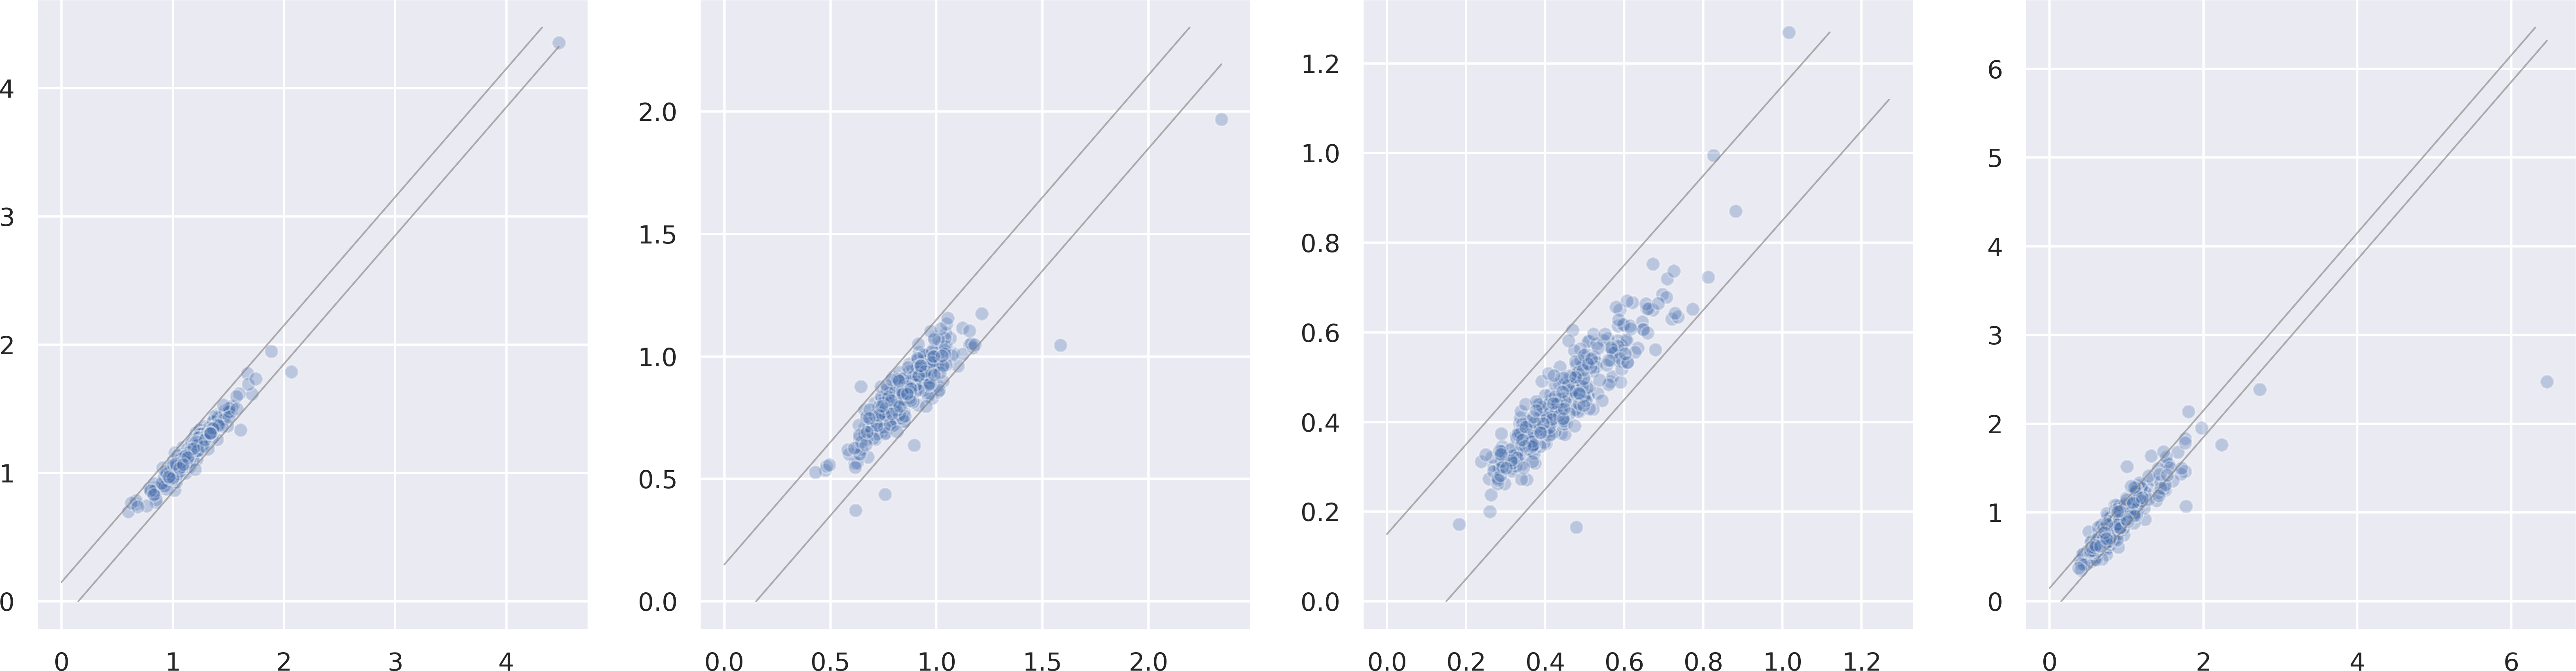
\includegraphics[width=\textwidth]{polyreg_keyvalfeat_reg_scatter_vred}
    \caption{\label{fig:polyreg_keyvalfeat_reg_scatter_vred} Scatter plots of \(Y_\text{true}\) (\(x\)-axis) versus \(Y_\text{pred}\) (\(y\)-axis) from the greatly reduced dataset comprising key values and features 1, 4 and 6, showing the polynomial regression model's damage prediction for features 2, 3, 5 and 7. Diagonal lines represent the \(\pm0.15\) tolerance for a hit.}
\end{figure}

\section{Summary}
The models and datasets implemented in this thesis have shown that the best way to predict damage from flight data is to perform a polynomial regression on key values --- values that describe important features of the data --- combined with damage values from neighbouring nodes. While this method is highly accurate and fulfils all criteria defined at the beginning of the research phase (see Section \ref{sec:conclusion}), its dependence on Cycle Counter damage values in the input data is somewhat disappointing.

Implementing the method at full scale with several thousand output values should allow an output to be generated within a few minutes on new flight data, but almost all of this time will consist of using the Cycle Counter to calculate the damage values used in the regression; producing output from the regression model alone is completed within a fraction of a second. This dependence on the Cycle Counter is a potential bottleneck.

It is also not a satisfying solution. The Cycle Counter computes its output by plugging \ac{ehm} data into an \ac{fe}-based response surface computed for the \ac{hpt} nodes. \ac{ml} and \ac{dl} models trained on the datasets without damage values are essentially an attempt to replicate this response surface in a model that computes the damage more efficiently. Using the Cycle Counter to predict other Cycle Counter values is an intermediate step that should be avoided. The challenge, in this case, is to find an approach that can replicate the response surface with sufficient accuracy.

If time series data is to be considered for future research in order to avoid depending on the Cycle Counter for input data, the downsampling process should be adjusted so as to minimise information loss. However, more input nodes result in more trainable parameters which, in turn, require a larger dataset to train. Therefore, it is essential to find a balance between minimising information loss while maximising data loss.

The results on time series data were highly comparable between \ac{cnn}-based networks and the simpler \ac{mlp}. Although the latter takes significantly less time to train due to its relative simplicity, this characteristic is also its limitation and it is unlikely to offer much room for optimisation. The Inception network was the state-of-the-art classifier of images in 2014 \cite[]{szegedy_going_2014}, but its accuracy has since been beaten by many other networks: there is room for improvement, therefore, in the InceptionTime model, too. \ac{cnn}s are consistently present in state-of-the-art models used for image classification and other computer vision tasks of similar complexity, so it is probable that they can, with sufficient research and suitable input data, offer a solution to replicating the response surface.

However, since this is likely to be a highly time-intensive task with no guaranteed solution, a more economical option is to investigate further descriptive values to use as input to a polynomial regression model. A preliminary analysis of \ac{dtw} (a means of quantifying the differences between two time series), carried out after the model implementation phases of this thesis, indicated that it may correlate highly with damage values. \ac{dtw} carries four potential advantages: firstly, it is designed to handle and take into account the temporal aspect of time series data; secondly, it can compute the distance between two time series of different lengths, making it suitable for use on the original, full-length \ac{ehm} data; thirdly, it can calculate this valuable data for all four \ac{ehm} parameters used in this thesis; and fourthly, it is computed very fast. % TODO: Time for plot next week?

This, therefore, should be one of the next steps for improving the accuracy of the proposed model. Should the Cycle Counter output values prove to be indispensable for reaching high levels of accuracy, \ac{dtw} can still be included to improve hit rates and \(R^2\).